\begin{appendices}
% Reset equation counter
\setcounter{equation}{0}
\renewcommand{\theequation}{\Alph{section}.\arabic{equation}}


%===========================================================================================
\section{Detailed Description of the Merger Tree algorithm}\label{app:detailed_mergertree}
%===========================================================================================


The merger tree code essentially consists of two steps:

\begin{enumerate}
	
	\item Create trees using progenitor data that was previously written to file and descendant data which is currently in memory.
    The clumps identified in the snapshot where the simulation currently is are treated as descendants, while the clumps from past snapshots are considered to be progenitors.
	
	\item Prepare and write data of current clumps to file. 
	This data will be the progenitor data in the following snapshot.
	
\end{enumerate}

Suppose the simulation is at the first snapshot that contains haloes.
As there are no progenitors available at this point, no trees can be made, so the code directly jumps to step 2:

\begin{itemize}
	
	\item For every clump, identify up to $n_{mb}$ tracker particles with minimal energy across all processing units.
	If a clump consists of less than $n_{mb}$ particles, then take the maximally available number of particles.
	
	\item Write the tracker particles of all processing units into a single shared file. 
	All processing units will read this file back in at the following snapshot.
	If past merged progenitors exist, also write these to (a different) shared file.
	
	\item Remove all clump finding data from memory and continue with the simulation.
	
\end{itemize}



At the next snapshot, the merger tree code will start once haloes have been identified.
This time, progenitors exist, so the code proceeds as follows:

\begin{itemize}
	
	\item Every processing unit reads in the progenitor data from the shared file of the previous snapshot.
	
	\item Process the progenitor data:
	\begin{itemize}
		\item Find which tracer particles are on each processing unit's domain by checking the particles' global ID.
		Each processing unit needs to know which tracer particles are currently on its domain.
		
		\item Find and communicate globally which processing unit is the ``owner'' of which progenitor (and past merged progenitor): 
		The owner of any progenitor is defined as the processing unit which has the most strongly bound particle of that progenitor within its domain.
		(Analogously as for the past merged progenitors, this particle is referred to as the ``galaxy particle'' of this progenitor.)
		
		\item Each processing unit henceforth only keeps track of the tracer particles that are on its domain.
		The rest are removed from memory.
	\end{itemize}
	
	\item Find links between progenitors and descendants: Essentially find ``which tracer particle ended up where'':
	
	\begin{itemize}
		\item After halo finding the halo to which any particle belongs is known.
		
		\item After reading in progenitor data the progenitor halo to which any tracer particle belonged is known.
		
		\item Each processing unit loops through all its local tracer particles.
		Using these two informations (in which halo the particle was and in which halo the particle is now) for every tracer particle, all descendant candidates for all progenitors are found and stored in a sparse matrix, where the rows correspond to progenitors and the columns are the descendants.
		The exact number of particle matches between a progenitor-descendant candidate pair is kept.
		Example: let $n_{mb}=200$. For progenitor with ID 1, a possible result would be to find 50 particles in descendant with ID 2, 120 particles in descendant with ID 7, 10 particles in descendant 3 and 20 particles that aren't in a halo at the current snapshot.
		
		
		\item The owner of progenitors gather and sum up all the matches found this way for that progenitor and then scatter them back to any processing unit that has at least one particle of that progenitor on their domain.
		(These are exactly the processing units that sent data to the owner of the progenitor in the first place.)
		
		\item After communications are done, create the transverse sparse matrix, where the rows are descendants and the columns are progenitors.
		These matrices will be used to loop through progenitor or descendant candidates.
		
	\end{itemize}
	
	\item Make trees:
	
	\begin{itemize}
		
		\item Obtain an initial guess for the main progenitors of every descendant and for the main descendant of every progenitor by finding the candidate that maximises the merit function \eqref{eq:merit}.
		
%		Finding the main progenitor or the main descendant is done almost identically:
%		Let $n_{A \cap B}$ be the number of particles shared by a progenitor $A$ and a descendant $B$, $m_>$ and $m_<$ be the bigger and the smaller mass between $A$ and $B$, respectively (e.g. if $m_A > m_B$: $m_> = m_A$).
%		The candidate for a main progenitor or main descendant which maximises the merit function\footnote{
%			Technically, this merit function should be normed, for example like this: 
%			$M_{A,B} = \frac{n_{A\cap B}}{n_{bm}} \left|\frac{m_{A,B}}{ m_>-m_<} \right|$. 
%			But $n_{mb}$ is a constant parameter, while $m_{A,B}$ can be chosen to be $m_A$ when evaluating descendant candidates for the progenitor $A$, and $m_B$ when evaluating progenitor candidates for the descendant $B$, which in both cases is independent of the candidate under evaluation and hence a redundant operation.
%		}
%		\begin{align*}
%		\mathcal{M} = \frac{n_{A\cap B}}{\left| 1 - \frac{m_>}{m_<} \right|}
%		\end{align*}
%		
%		The factor $| 1 - \frac{m_>}{m_<} |^{-1}$ is chosen to favour pairings of similar mass and suppress big jumps in mass of a halo between two snapshots. 
		
		\item Loop to establish matches:
		
		A main progenitor-descendant pair is established when the main progenitor of a descendant is the main descendant of said progenitor, or in pseudocode:
		\begin{verbatim}
		match = (main_prog(idesc)==iprog) && (main_desc(iprog) == idesc)
		\end{verbatim}
		
		
		While there are still descendants without a match and still progenitor candidates left for these descendants:
		
		\begin{itemize}
			
			\item Loop through all descendant candidates of progenitors without a match, unless you find a match.
			
			\item For all descendants without a match: Switch to the next best progenitor candidate as current best guess.
			
		\end{itemize}
		
		The loop ends either when all descendants have a match, or if descendants run out of candidates.
		
		If a progenitor hasn't found a match, assume it merged into its best descendant candidate.
		
		\item Add merged progenitors to the list of past merged progenitors.
		
		\item If there are descendants that still have no main progenitor: Try finding a progenitor from an older, non-consecutive snapshot.
		Past merged progenitors are tracked by one particle, their ``galaxy particle''. 
		All particles of the descendant under investigation are checked for being a galaxy particle of a past merged progenitor.
		The most strongly bound galaxy particle will be considered the main progenitor of the descendant under consideration.
		If a match is found, the past merged progenitor is removed from the list of past merged progenitors.
		
		\item Descendants that still haven’t found a progenitor at this point are deemed to be newly formed.
		
	\end{itemize}
	
	\item The results are written to file, and the code goes on to the previously described step 2.
	
\end{itemize}






















%=======================================================================================================================================================
\section{Testing Parameters of the Merger Tree Algorithm: Results Distinguishing Between Haloes and Subhaloes }\label{app:halo-subhalo-mtree-evals}
%=======================================================================================================================================================

In this section, the results for the evaluations of the merger tree algorithm parameters,  as described in section \ref{chap:tests} are given, including the distinction between subhaloes and haloes.

Displacement statistics (eq. \ref{eq:displacements}) are shown in figure \ref{fig:displacements-subhalo}, logarithmic mass growths (eq. \ref{eq:massgrowth}) and mass growth fluctuations (eq. \ref{eq:massfluct}) are shown in figure \ref{fig:mass-growth-and-flucts-saddle-vs-nosaddle-subhalo} for the \sad/\nosad\ comparison and in figure \ref{fig:mass-growth-and-flucts-ntracers-subhalo} for varying number of tracer particles $n_{mb}$.


\begin{figure}[H]
	\centering
		\minipage[t]{0.49\textwidth}
		\centering
		\includegraphics[width=\textwidth]{images/saddle-vs-nosaddle-subhalo/displacements.pdf}
	\endminipage%\hspace{.1cm}
	\hspace*{\fill}
	%
	\minipage[t]{0.49\textwidth}
		\centering
		\includegraphics[width=\textwidth, keepaspectratio]{images/ntracers-subhalo/displacements.pdf}%
	\endminipage\hspace*{\fill} 
	\caption{
		Distribution of the displacements for progenitor - descendant pairs with masses above $5\cdot 10^{11}\msol$ throughout the entire simulation for the halo catalogue influencing parameters: 
		whether subhalo particles are included (\inc) or excluded (\exc) in the clump mass of satellite haloes, and whether to consider particles which might wander off into another clump as bound (\nosad) or not (\sad) are shown in the left plot.
		The results for varying numbers of clump tracer particles, $n_{mb}$, are shown in the right plot.
		Solid lines are for haloes, dashed lines are for subhaloes.
		The distributions are computed as a histogram which is normalised by the total number of events found.
	}%
	\label{fig:displacements-subhalo}
\end{figure}



\begin{figure}[H]
	\centering
	\includegraphics[width=\textwidth, keepaspectratio]{images/saddle-vs-nosaddle-subhalo/mass_growth_and_fluctuation.pdf}%
	\caption{
		Logarithmic mass growth and mass growth fluctuation distributions for progenitor - descendant pairs or three consecutive nodes in a branch, respectively, with masses above $5\cdot 10^{11}\msol$ throughout the entire simulation for the halo catalogue influencing parameters: 
		whether subhalo particles are included (\inc) or excluded (\exc) in the clump mass of satellite haloes, and whether to consider particles which might wander off into another clump as bound (\nosad) or not (\sad).
		The distribution is computed as a histogram which is normalised by the total number of events found.
		The upper row contains the results for haloes, the lower for subhaloes.
	}%
	\label{fig:mass-growth-and-flucts-saddle-vs-nosaddle-subhalo}
\end{figure}



\begin{figure}[H]
	\centering
	\includegraphics[width=\textwidth, keepaspectratio]{images/ntracers-subhalo/mass_growth_and_fluctuation.pdf}%
	\caption{
		Logarithmic mass growth and mass growth fluctuation distributions for progenitor - descendant pairs or three consecutive nodes in a branch, respectively, with masses above $5\cdot 10^{11}\msol$ throughout the entire simulation for varying numbers of clump tracer particles $n_{mb}$.
		The upper row contains the results for haloes, the lower for subhaloes.
	}%
	\label{fig:mass-growth-and-flucts-ntracers-subhalo}
\end{figure}






















%=================================================================
\section{Stellar Mass Functions at Mean Redshift vs Average Over Redshift Interval}\label{app:smf_variations}
%=================================================================

Figure \ref{fig:smf-central-average} shows the obtained stellar mass functions $\Phi(M_*)$ over redshift intervals of the \gsmall\ simulation for both the snapshot with redshift closest to the central redshift of the interval used for observational data and the average SMF computed over all snapshots with redshift within the redshift interval.
The differences are negligible.




\begin{figure}[H]
	\centering
	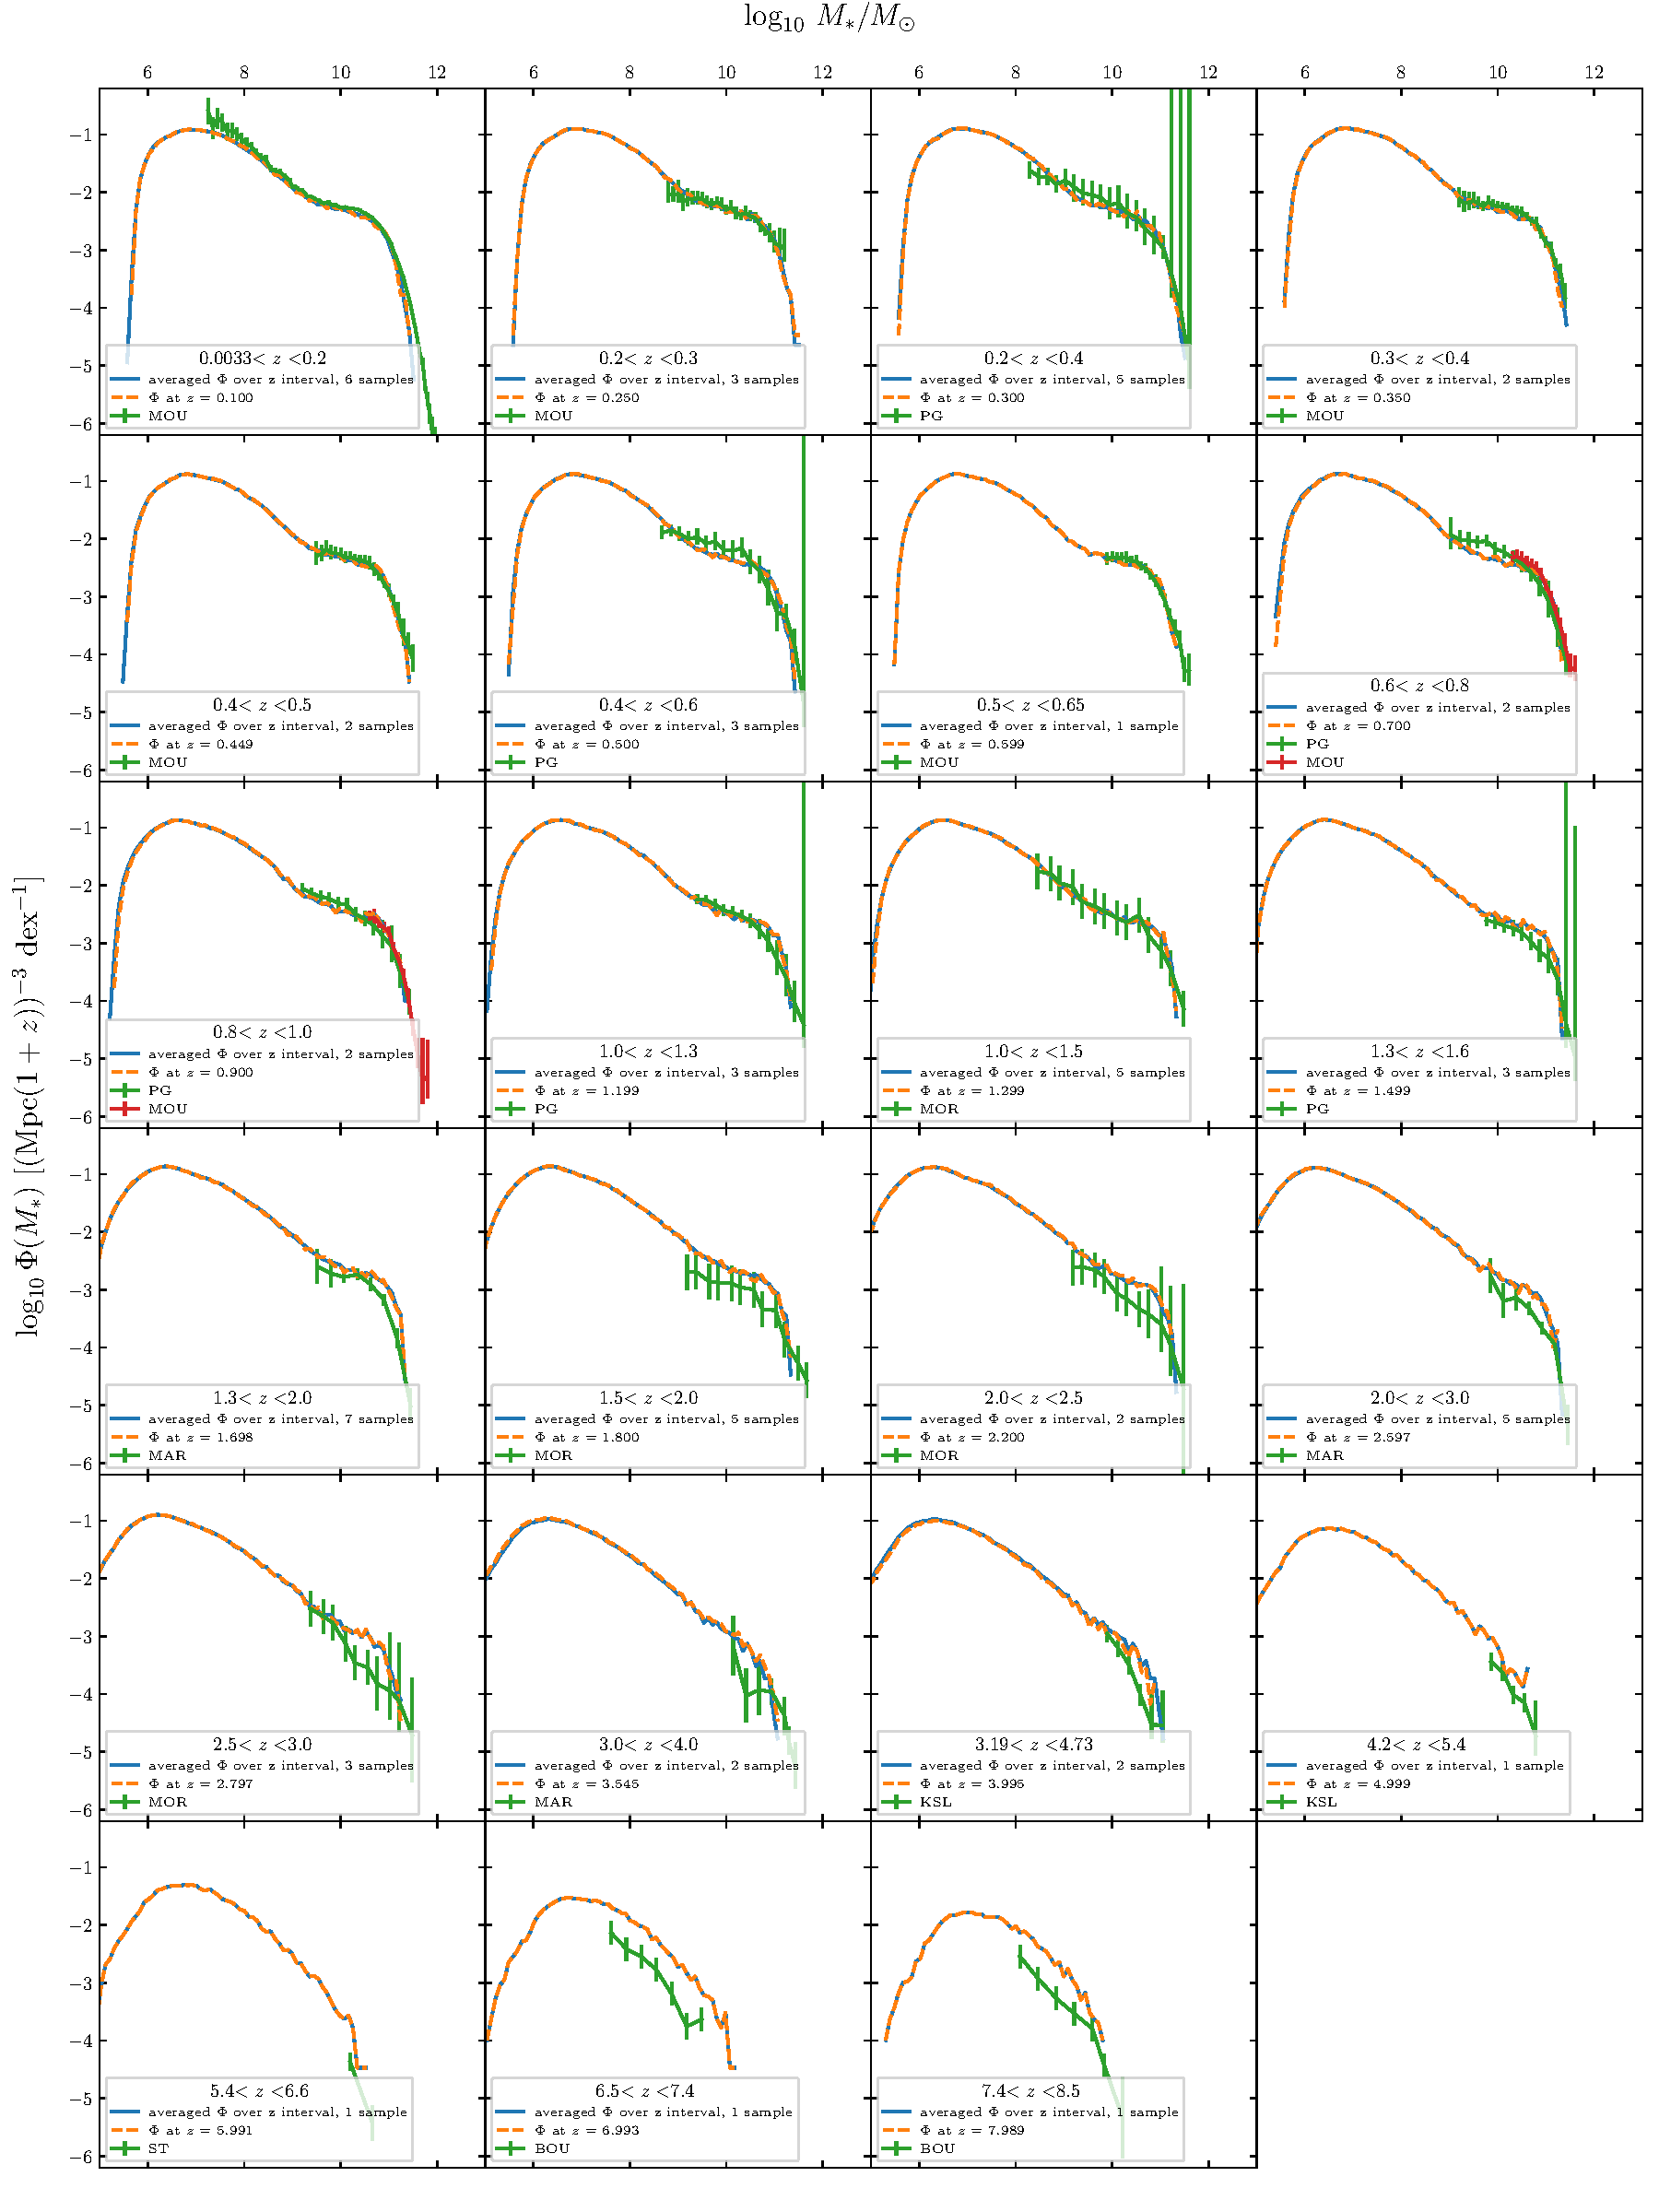
\includegraphics[width=\textwidth]{images/smf/smf-G69-central-average.pdf}%
	\caption{
		Obtained stellar mass functions $\Phi(M_*)$ of central galaxies for the \gsmall\ simulation datasets described in \ref{chap:sim_galaxy} both averaged over the redshift interval of the observational data and from a single snapshot closest to the centre of the interval compared to observed stellar mass functions.
		The abbreviations used for observational data are listed in table \ref{tab:obs_smf}.
	}%
	\label{fig:smf-central-average}
\end{figure}




\end{appendices}